The requeriments of the ultrapure water system are:

\begin{enumerate}

\item{} A high degree of purification of the processed water sample, reducing its conductivity by approximately two orders of magnitude (from $1000~\mu$S$/\cm$ to $10~\mu$S$/\cm$)

\item{} Low maintenance (low cost  and low manpower)

\item{} To manage probes and valves by software.
\end{enumerate}

The LARUEX laboratory in Extremadura, one of the six collaborators of the TRITIUM experiment, has designed, developed and built the ultrapure water system, a scheme of which is shown in Figure \ref{fig:WPSScheme}.

\begin{figure}[htbp]
\centering
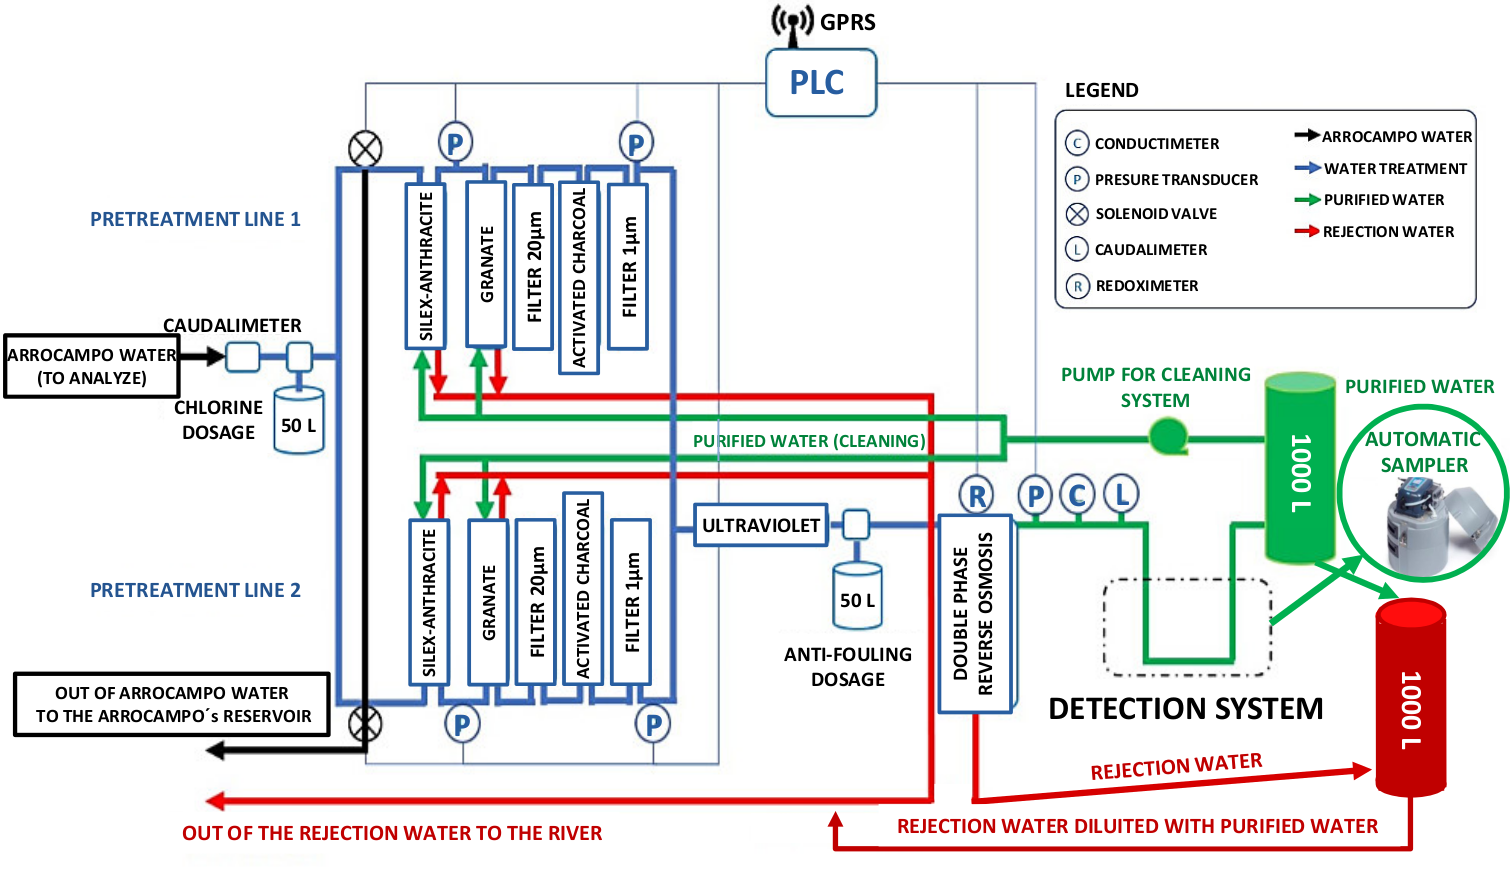
\includegraphics[scale=0.25]{3DesignPrinciples/33UltraPureWaterSystem/SchemeUltraPureWaterSystem.png}
\caption{Scheme of water purification system.\label{fig:WPSScheme}}
\end{figure}

This system is installed in the Arrocampo dam and consists of four different stages:

\begin{enumerate}
\item{} The raw water from the Tagus river passes through two different filters, the first made of silex-anthracite and the second of garnet, with which a rough filtering is made (the largest particles are eliminated). This system has two parallel lines and implements self-cleaning by injecting ultrapure water in the opposite direction.

\item{} The outlet water sample of the first stage, called fine filtration stage, passes through a $20~\mu\meter$ filter (formed by a synthetic mesh) and activated charcoal filters (one per line) that remove chlorine and iron particles.

\item{} The outlet water of the second stage passes through a super-fine filtering consisting of a $1~\mu\meter$ filter, formed of a dense polypropylene mesh and UV lamps. The first filter removes all the particles up to diameters of $1~\mu\meter$ and the UV lamps remove the organic matter present in the sample.

\item{} Finally, the water is introduced in the last stage, double-phase reverse osmosis, that reduces the conductivity of the water to about $5~\mu$S$/\cm$. It was verified that a conductivity of $10~\mu$S$/\cm$ is achieved with only one module of reverse osmosis, enough for the needed conditions. Therefore, only one module of reverse osmosis is used, reducing the power consumption of the system.

\end{enumerate}

As a result of the purification process, besides the ultrapure water that is introduced into the TRITIUM detector, a rejection water is produced,  which contains the particles extracted from the ultrapure water that results in conductivities greater than the original water.

The ultrapure water system is able to process up to $0.850~\meter^3/\hour$ with a single line operating or $1.480~\meter^3/\hour$ with both, greatly outperforming the requirements of the tritium detector. 

The software used for remote controlling the ultrapure water system is Siemens PLC, that gives information such as the state of the valves, the reading of pressure probes and the amount of water production in real time. 

The appendix \ref{App:UltraPureWaterSystem} contains several pictures of different parts of this system, installed in Arrocampo dam.